\documentclass[a4paper,11pt]{jsarticle}

\usepackage[top=30truemm,bottom=30truemm,left=25truemm,right=25truemm]{geometry}
\usepackage{amsmath,amsfonts}
\usepackage{mathcomp}
\usepackage{textcomp}
\usepackage{bm}
\usepackage[dvipdfmx]{graphicx}
\usepackage{booktabs}
\usepackage{array}
\usepackage{multirow}
\usepackage{here}
\usepackage{array}
\usepackage{tabu}
\usepackage{wrapfig}
\usepackage{siunitx}
\usepackage{subcaption}

\begin{document}

\title{光学顕微鏡と走査型電子顕微鏡による形態観察}
\author{1522063 手塚裕貴 \\共同実験者 1522B02 中村洸太}
\date{実験日 2023 年 5月 23日, 30日}
\maketitle

\begin{abstract}
  この実験の目的は主に二つある。一つ目は、光学顕微鏡と走査型電子顕微鏡の性能と特徴について比較し、解像度、色再現性、焦点深度の観点から違いを考察することである。二つ目は、絶縁性試料と伝導性試料における加速電圧の影響を調べることである。
  これらの目的に基づいて、以下の二つの実験を行った。実験1では、伝導性試料である回析格子を走査型電子顕微鏡を用いて撮影した。
  実験2では、絶縁性試料であるレコード盤を光学顕微鏡と走査型電子顕微鏡の二つで撮影した。走査型電子顕微鏡で撮影する際は、加速電圧を変化させて撮影した。その結果、以下の二つのことが得られた。一つ目は、導電性試料では、加速電圧を高くすると解像度が向上するが、絶縁性試料では加速電圧を高くすると解像度が低下する。一般に、入射電子のエネルギーを上昇させると二次電子のエネルギーも上昇する為、表面凹凸に応じた二次電子の放出量の差が大きくなる。その結果、濃淡がはっきりと映し出される。しかし、絶縁性試料の場合は、照射された電子が試料表面に過剰にたまってしまう為、加速電圧を高くするほど鮮明さが欠けてしまうと考えられる。\\
  二つ目として、光学顕微鏡では焦点深度が限られるが、走査型電子顕微鏡では電子線の波長が短く絞りが小さいため、焦点深度が大きくなることが観察された。
\end{abstract}

\section{Introduction}

\subsection{走査型電子顕微鏡}
走査型電子顕微鏡(Scanning Electron Microscope: SEM)は図1に示すように、主に電子を放出する電子銃、放出された電子を収束させる電子レンズ、収束された電子線を資料表面の観察領域に照射するための偏光器、試料から散乱する電子を検出する検出器からなる。


\begin{wrapfigure}{l}[0pt]{0.5\textwidth}
  \centering
  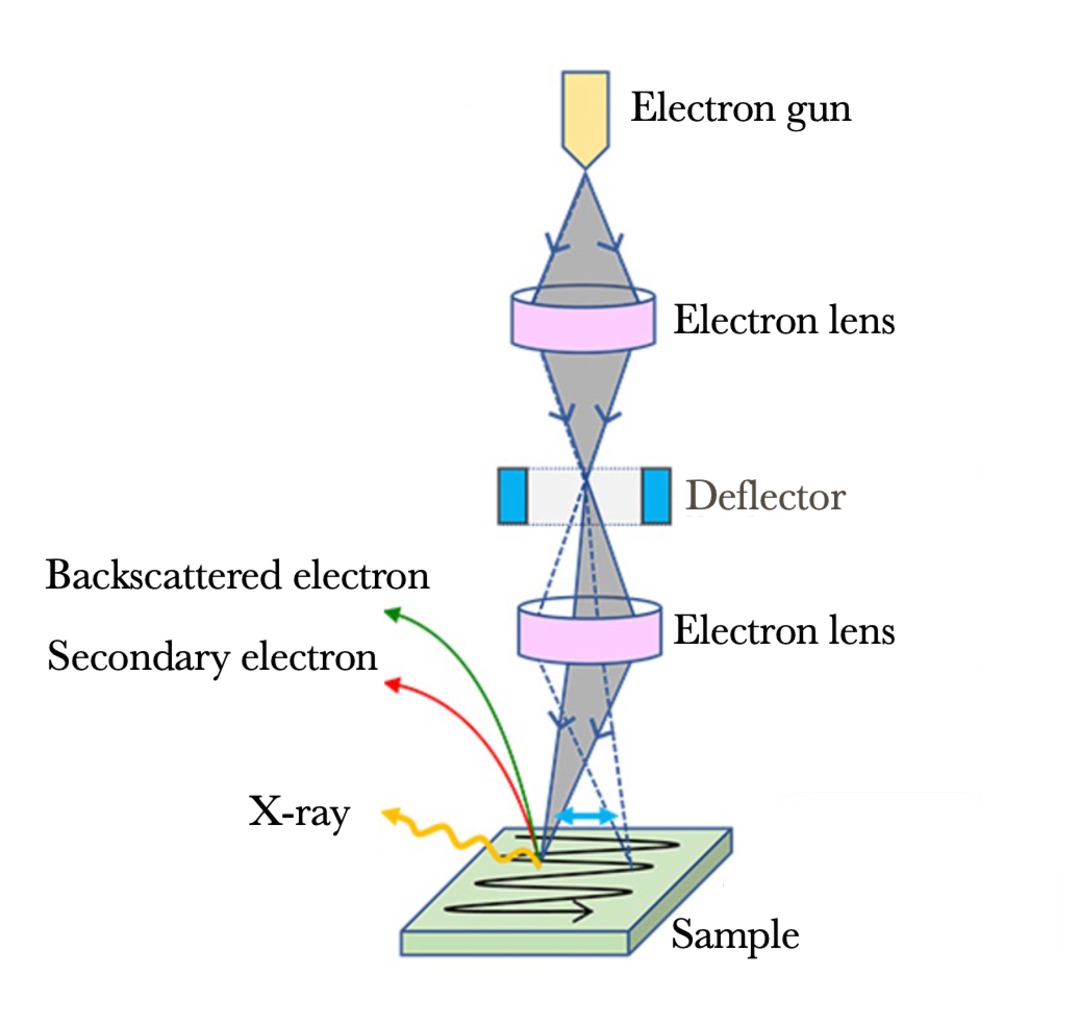
\includegraphics[width=0.4\textwidth]{figs/sen.pdf}
  \caption{SENの概要図}
  \label{fig:arc}
\end{wrapfigure}
代表的な電子銃として熱電子型と電界放出型がある。熱電子型はタングステンフィラメントへの通電加熱で電子を放出させる方式である。一方、電界放出型は単結晶の針の先端への強い電場印加で電子を引き出す方式である。本実験で使用する走査型電子顕微鏡(JSM-6390)は熱電子型の電子銃を使用している。
電子銃から放出された電子は電場により加速され電子レンズに入る。電子レンズは電子線を収束させるための装置である。電子レンズは光学顕微鏡の凸レンズのような役割を果たし、電場や磁場により加速電子を収束させる。収束された電子は偏向器を用いて観察領域を一筆書きで塗るように端から端まで照射される。試料に照射された電子は、試料表面内部に入射されるが、いくつかの電子は試料表面から散乱される。
表面から散乱する電子には、入射した電子がそのまま反射した反射電子と、試料中にあった電子が叩き出されて出てきた二次電子の2種類がある。
二次電子は凹凸に応じて表面から出てくる量が増減するため、電子線を走査しながら二次電子の量を検出することで、試料表面の凹凸情報を反映した画像を得ることができる。
切り立った角度の大きい場所から散乱する二次電子は多く、平坦な場所から散乱する二次電子は少ないため(エッジ効果)、二次電子の量が多い領域ほど白く画像化することで、白黒の濃淡で凹凸を表現することができる。
一方、反射電子は重い原子からは多く反射されるため、試料を構成する元素に応じた画像を得ることもできる。

二次電子を放出する際にはX線も放出されるが、そのX線が持つエネルギーを調べることで、特定の元素の種類や量の分布を可視化することができる。

\begin{figure}[H]
  \centering
  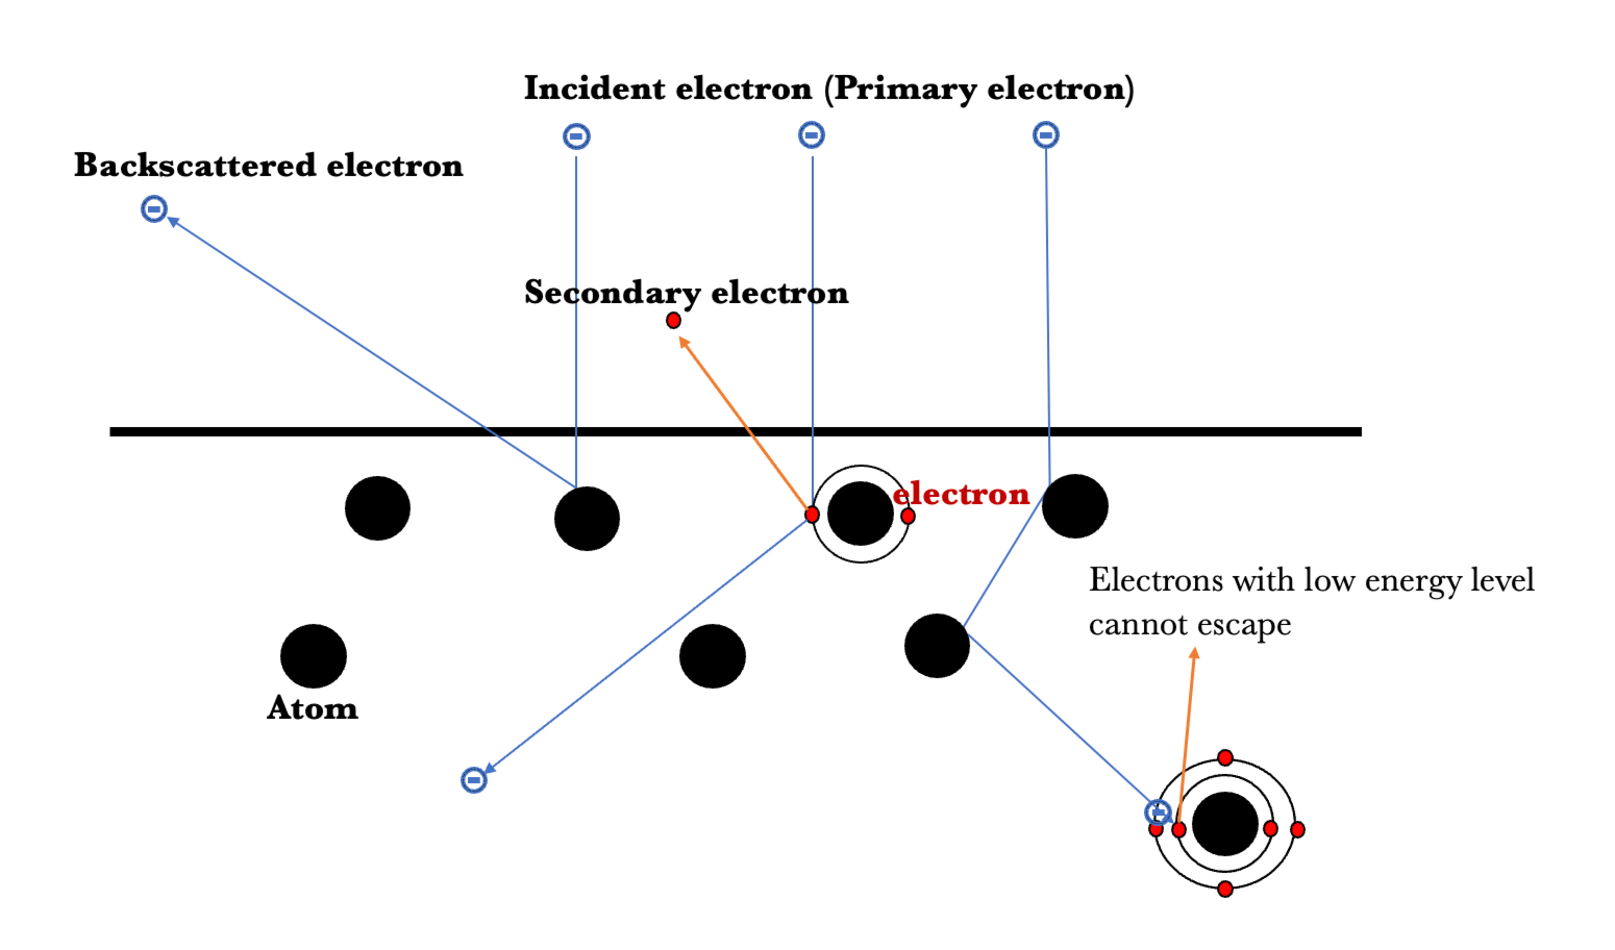
\includegraphics[width=0.7\textwidth]{figs/electron.pdf}
  \caption{入射電子の行方}
\end{figure}
二次電子は反射電子よりもエネルギーが小さく試料の深く(数十nm以下)から試料外部への脱出は難しく、
表面近傍の情報を多く含んでいるとされている。
\section{Methods}
 [実験装置]\\
・走査型電子顕微鏡(JSM-6390)\\
・走査型電子顕微鏡用治具一式\\
・走査型電子顕微鏡簡易操作マニュアル\\
・光学顕微鏡\\
・光学顕微鏡用PC\\
・光学顕微鏡写真取り込みマニュアル\\
・観察試料(試料1:回折格子、試料2:レコード盤)
\\

\subsection{走査型電子顕微鏡による回析光子の観察}
1. 回折格子をピントを合わせながら10000倍で撮影し、その後7500倍、5000倍、2500倍を撮影した。また、各倍率について30°の傾斜をつけたものとつけないものの両方の像を撮影した。さらに測長機能を用いて、jグレーティングの格子間隔を求めた。\\
\indent 2. 倍率10000倍の時に、加速電圧を5kv、10kv、15kv、20kvに変えて観察し、撮影した。
\subsection{光学顕微鏡と走査型電子顕微鏡によるレコード盤の観察}
1. 光学顕微鏡を用いて、レコード盤および対物微尺を200倍で撮影し、同一倍率で撮影した対物微尺の目盛からレコード盤の溝の間隔を求めた。\\
\indent 2. 走査型電子顕微鏡を用いて、同一のレコード試料を200倍で撮影した。さらに、レコード盤の溝を測長機能を用いて測定した。

\section{Results}
\subsection{走査型電子顕微鏡による観察}
\subsubsection{回析格子の観察}
回析格子を、2500倍、5000倍、7500倍、10000倍で観察した。また、各倍率について30°の傾斜をつけたものとつけないものの両方の像を撮影した。撮影した画像を図3$\sim$図10に示す。\\
\begin{figure}[H]
  \begin{minipage}{0.5\hsize}
    \begin{center}
      \includegraphics[width=0.85\textwidth]{figs/0523/kaisetukousi/2500_20kV.pdf}
    \end{center}
    \caption{回析格子 2500倍 20kV 傾斜なし}
  \end{minipage}
  \begin{minipage}{0.5\hsize}
    \begin{center}
      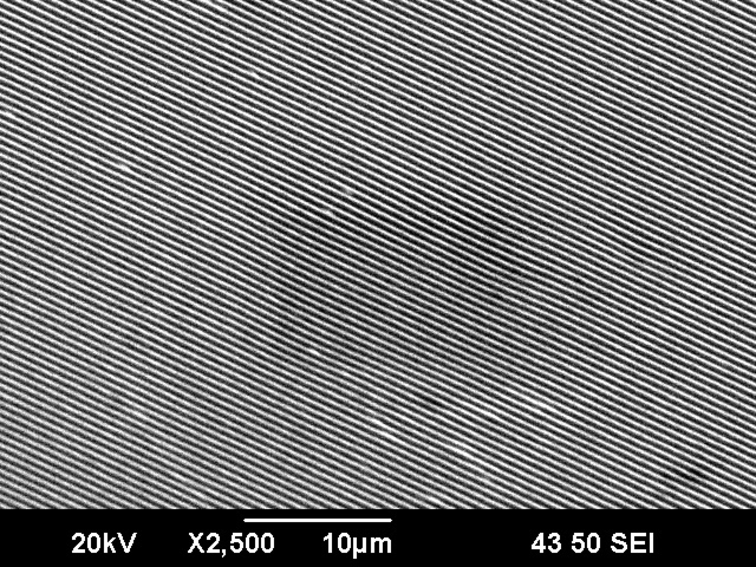
\includegraphics[width=0.85\textwidth]{figs/0523/kaisetukousi/2500_20kV_60.pdf}
    \end{center}
    \caption{回析格子 2500倍 20kV 傾斜60°}
  \end{minipage}
\end{figure}
\begin{figure}[H]
  \begin{minipage}{0.5\hsize}
    \begin{center}
      \includegraphics[width=0.85\textwidth]{figs/0523/kaisetukousi/5000_20kV.pdf}
    \end{center}
    \caption{回析格子 5000倍 20kV 傾斜なし}
  \end{minipage}
  \begin{minipage}{0.5\hsize}
    \begin{center}
      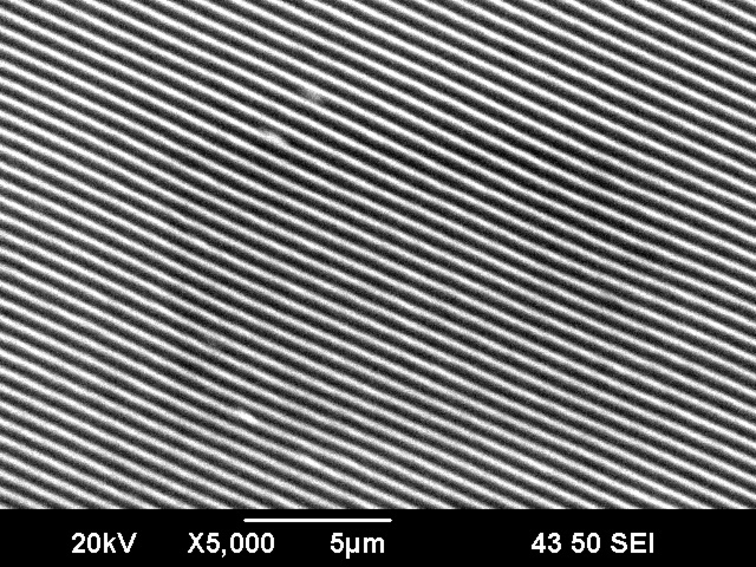
\includegraphics[width=0.85\textwidth]{figs/0523/kaisetukousi/5000_20kV_60.pdf}
    \end{center}
    \caption{回析格子 5000倍 20kV 傾斜60°}
  \end{minipage}
\end{figure}
\begin{figure}[H]
  \begin{minipage}{0.5\hsize}
    \begin{center}
      \includegraphics[width=0.85\textwidth]{figs/0523/kaisetukousi/7500_20kV.pdf}
    \end{center}
    \caption{回析格子 7500倍 20kV 傾斜なし}
  \end{minipage}
  \begin{minipage}{0.5\hsize}
    \begin{center}
      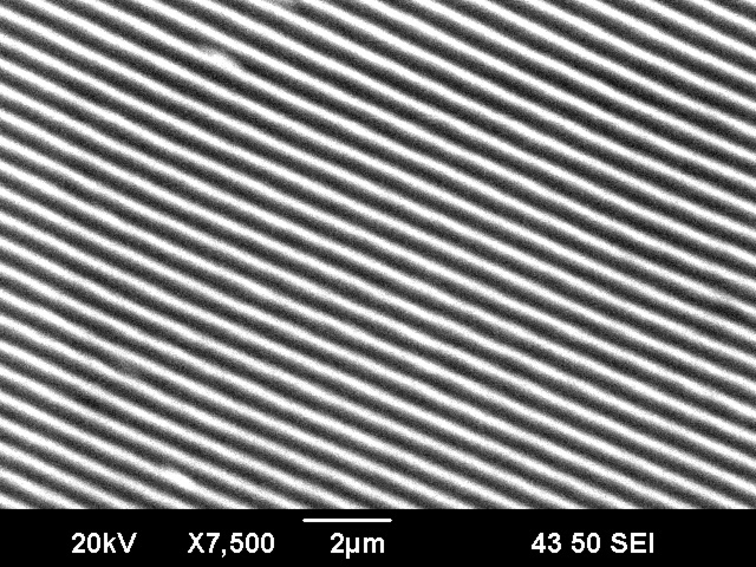
\includegraphics[width=0.85\textwidth]{figs/0523/kaisetukousi/7500_20kV_60.pdf}
    \end{center}
    \caption{回析格子 7500倍 20kV 傾斜60°}
  \end{minipage}
\end{figure}
\begin{figure}[H]
  \begin{minipage}{0.5\hsize}
    \begin{center}
      \includegraphics[width=0.85\textwidth]{figs/0523/kaisetukousi/10000_20kV_re.pdf}
    \end{center}
    \caption{回析格子 10000倍 20kV 傾斜なし}
  \end{minipage}
  \begin{minipage}{0.5\hsize}
    \begin{center}
      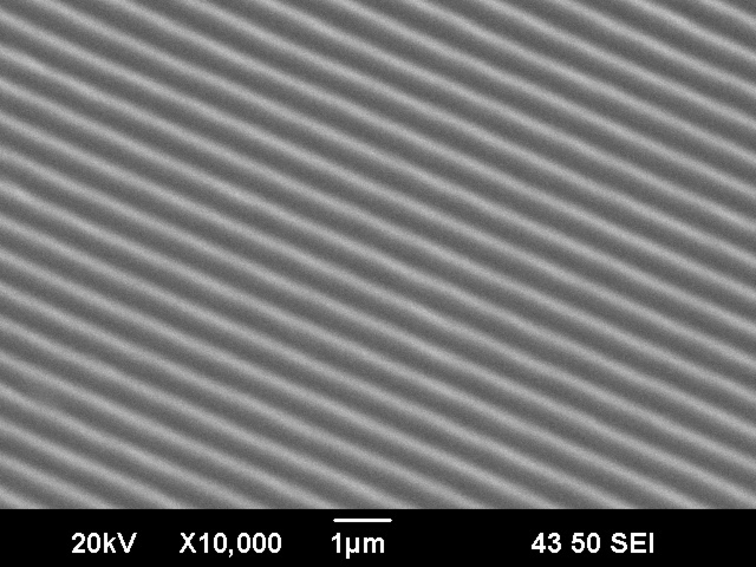
\includegraphics[width=0.85\textwidth]{figs/0523/kaisetukousi/10000_20kV_60.pdf}
    \end{center}
    \caption{回析格子 10000倍 20kV 傾斜60°}
  \end{minipage}
\end{figure}
図9よりグレーティングの格子間隔は$1.06\pm 0.02$ \textmu mであった。\\
図3$\sim$図6を見ると、写真中央には黒い影のようなものが確認できる。
これは、高倍率での長時間の電子線照射により、試料表面の炭化痕が捕捉された結果であると考えられる。\\

\subsubsection{加速電圧の変化による回析格子の観察}
倍率10000倍について、加速電圧を5kV、10kV、15kVに変えて撮影した。画像を図11$\sim$図14がその結果である。\\
\begin{figure}[H]
  \begin{minipage}{0.5\hsize}
    \begin{center}
      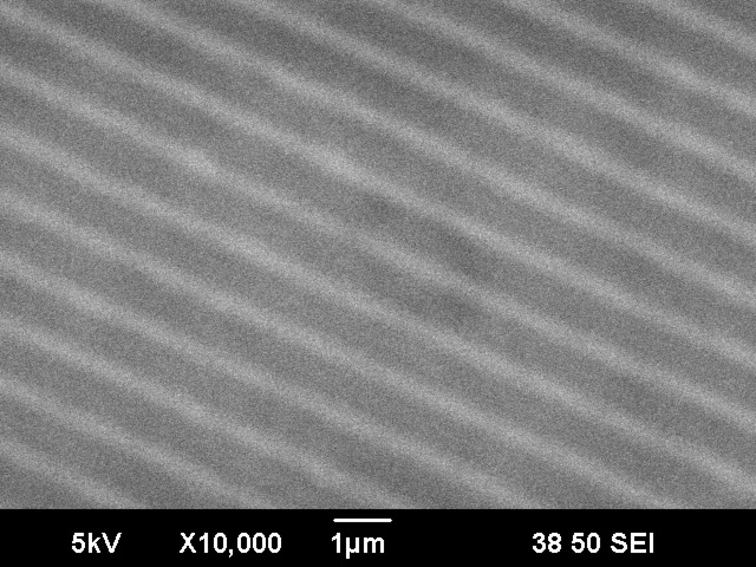
\includegraphics[width=0.85\textwidth]{figs/0523/kaisetukousi/10000_5kv.pdf}
    \end{center}
    \caption{回析格子 10000倍 5kV 傾斜なし}
  \end{minipage}
  \begin{minipage}{0.5\hsize}
    \begin{center}
      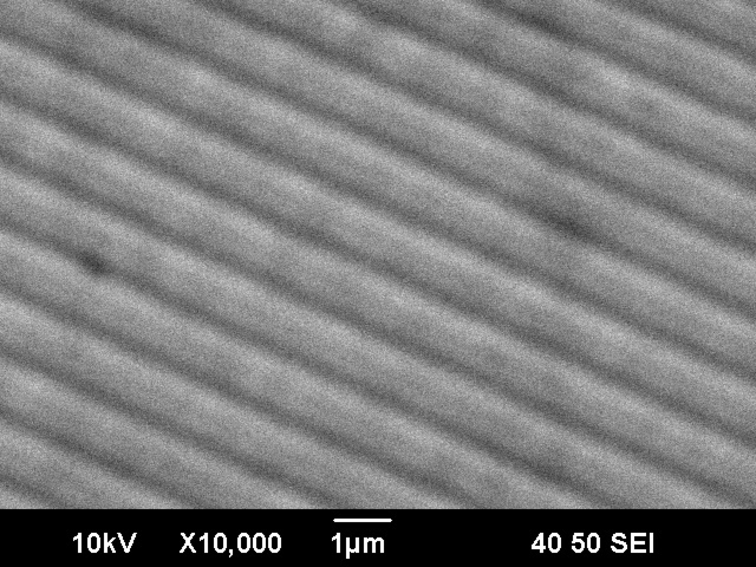
\includegraphics[width=0.85\textwidth]{figs/0523/kaisetukousi/10000_10kv.pdf}
    \end{center}
    \caption{回析格子 10000倍 10kV 傾斜なし}
  \end{minipage}
\end{figure}
\begin{figure}[H]
  \centering
  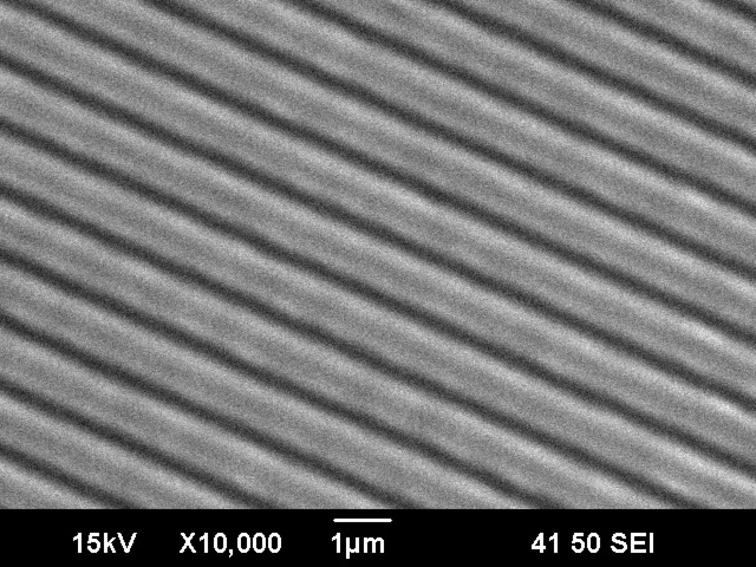
\includegraphics[width=0.425\textwidth]{figs/0523/kaisetukousi/10000_15kv.pdf}
  \caption{回析格子 10000倍 15kV 傾斜なし}
\end{figure}
図11$\sim$図13から分かるように、加速電圧が上がるにつれて白黒の濃淡がはっきりと映し出されている。
これは、入射電子のエネルギーが上昇すると、二次電子のエネルギーも上昇する為、表面凹凸に応じた二次電子の放出量の差が大きくなったことが原因であると考えられる。\\
\subsection{光学顕微鏡との比較}
\subsubsection{光学顕微鏡によるレコード盤の観察}
光学顕微鏡を用いて、レコード盤および反射用対物微尺を200倍で撮影した。
\begin{figure}[H]
  \centering
  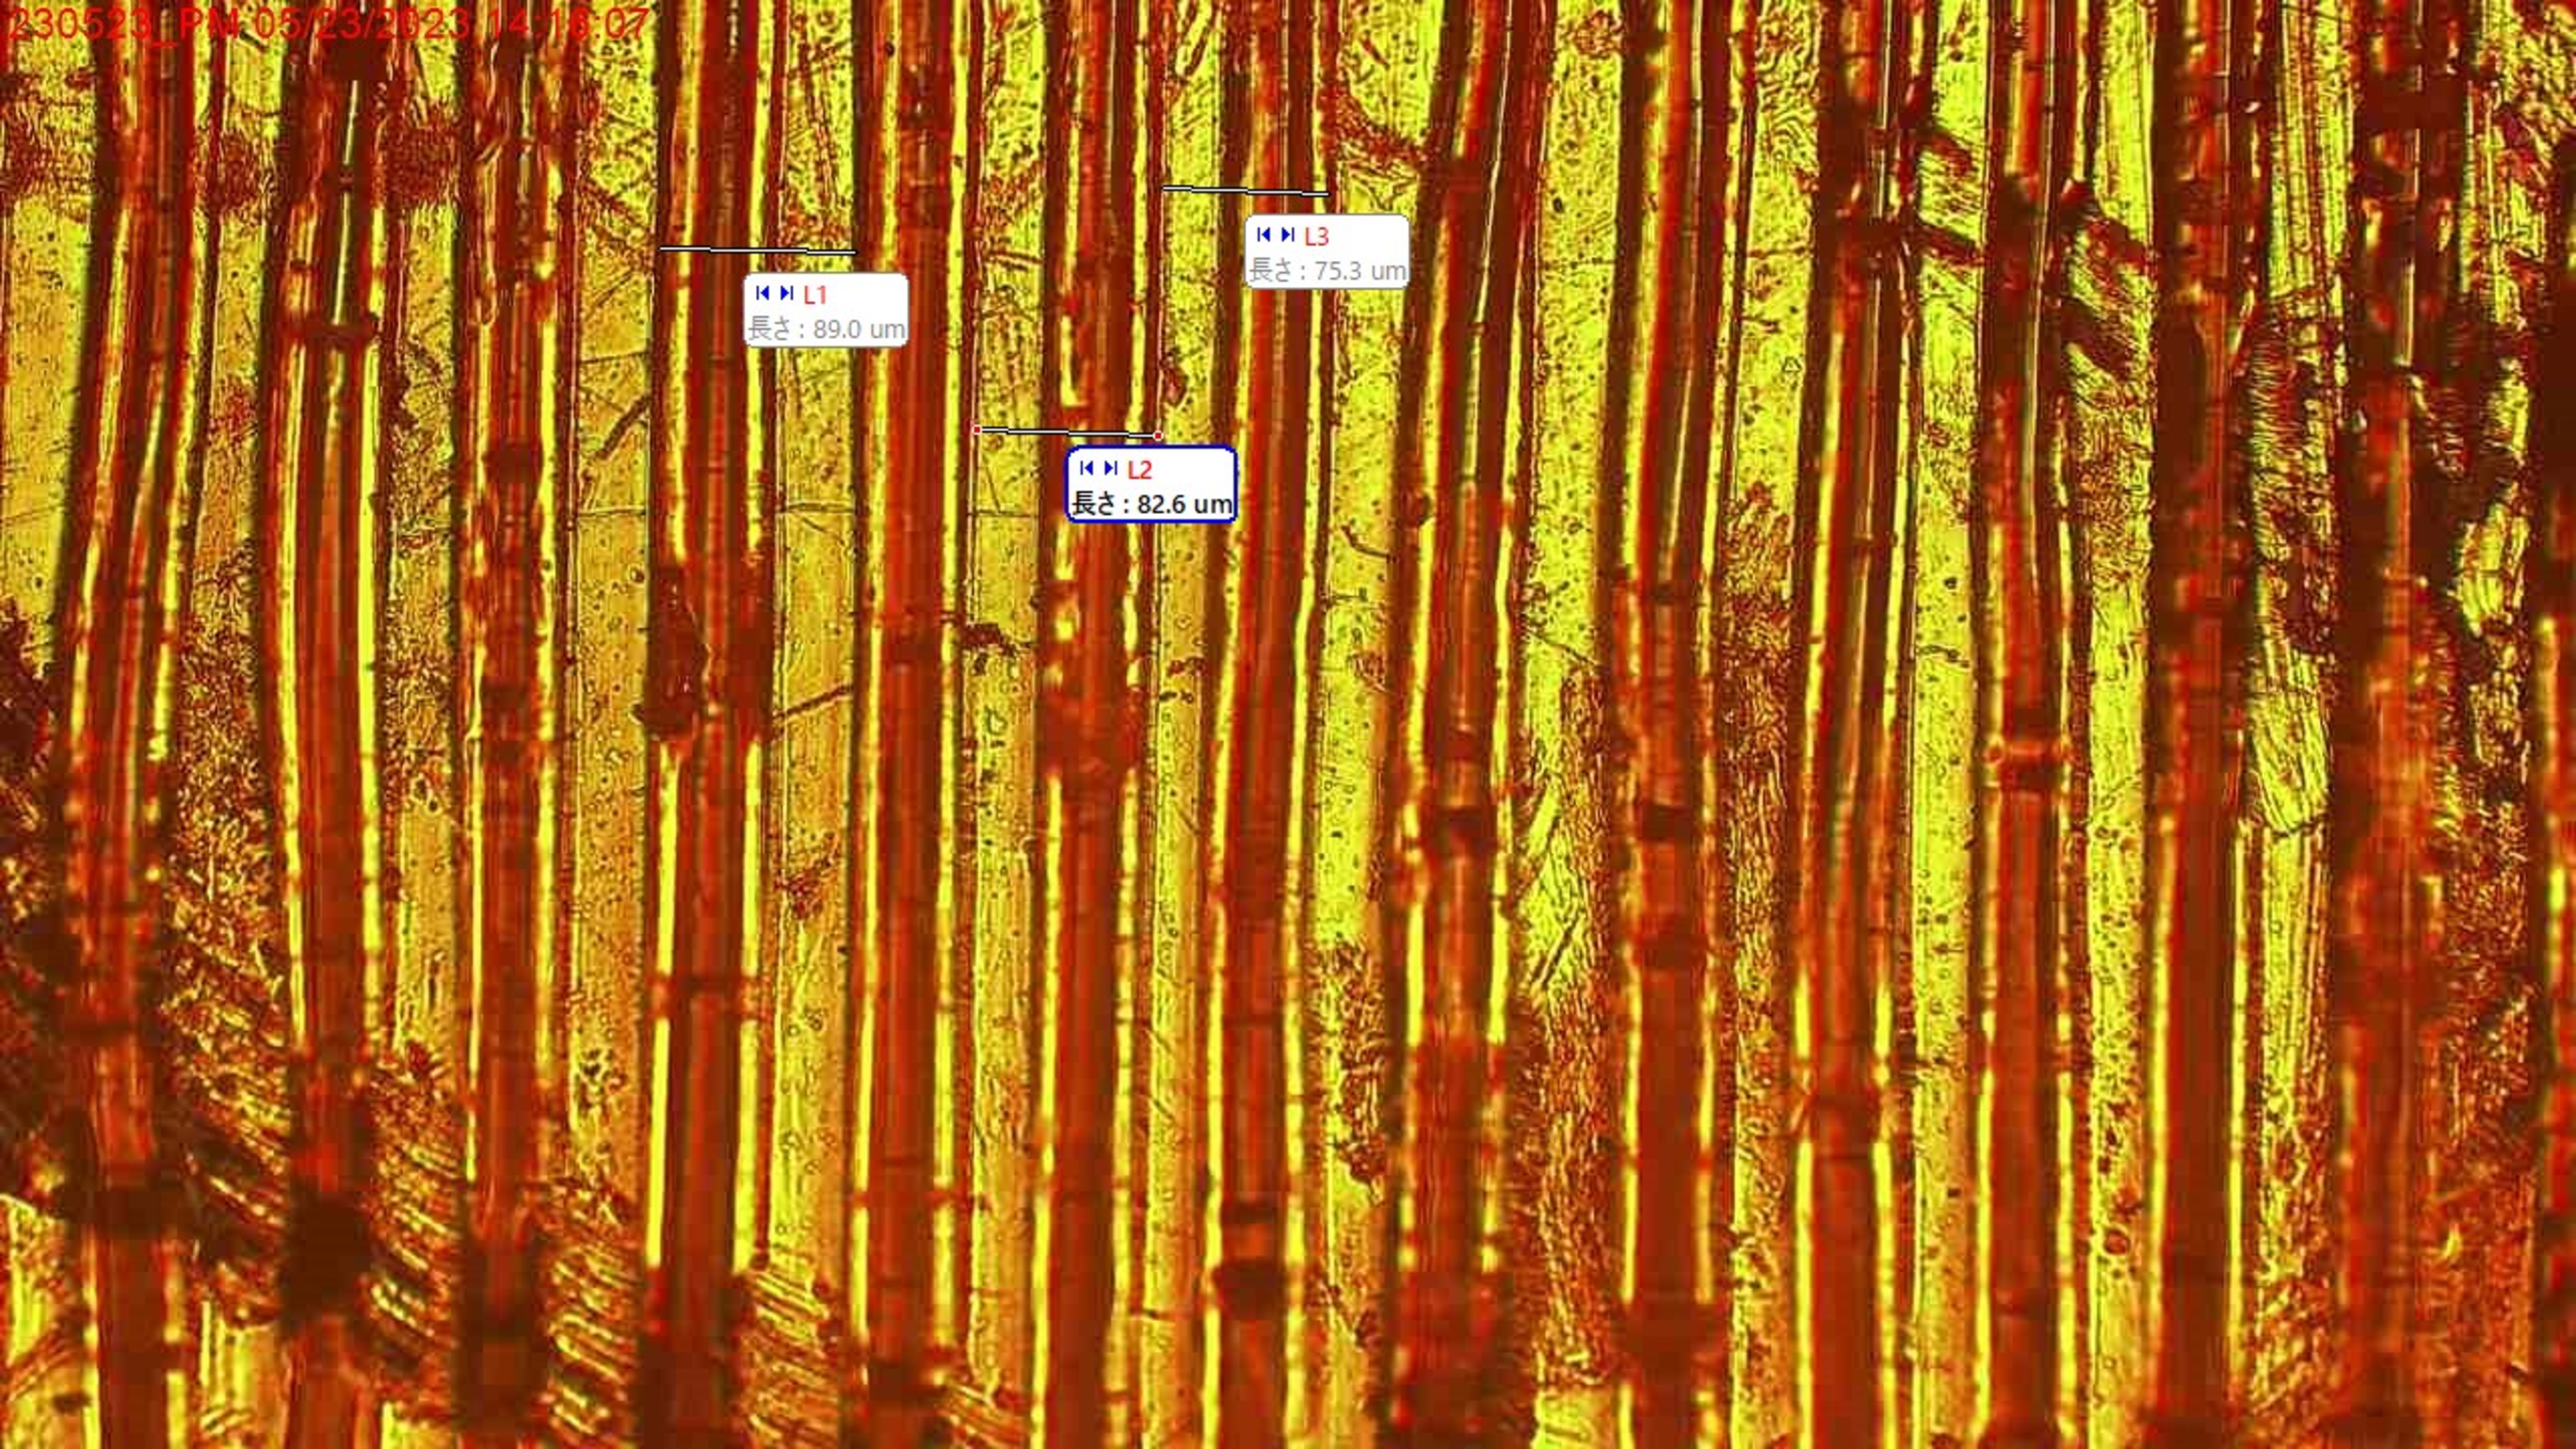
\includegraphics[width=0.425\textwidth]{figs/0523/record.pdf}
  \caption{レコード盤 200倍}
\end{figure}
同倍率で撮影した対物微尺の目盛を用いて、レコード盤の溝の間隔を測定した結果、$82.3\pm 2.5$ \textmu mであった。\\
\subsubsection{走査型電子顕微鏡によるレコード盤の観察}
走査型電子顕微鏡を用いて3.2.1と同一の試料を200倍で撮影した。\\

\begin{figure}[H]
  \begin{minipage}{0.5\hsize}
    \begin{center}
      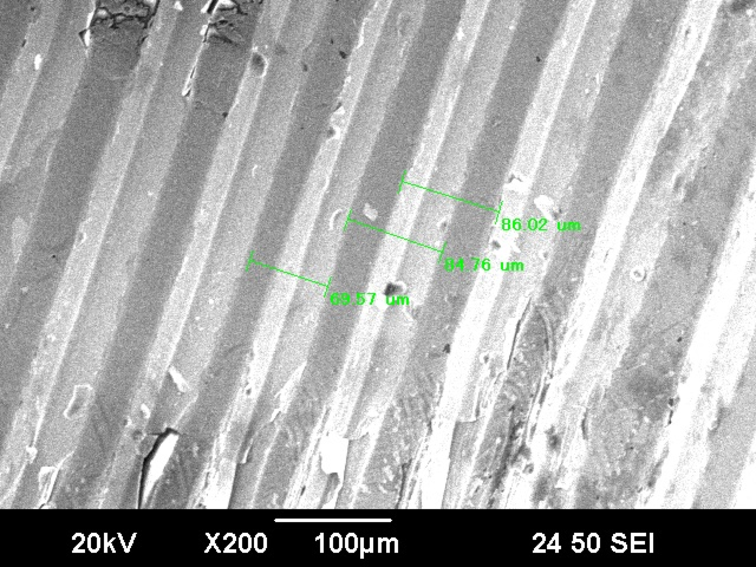
\includegraphics[width=0.85\textwidth]{figs/0523/record2/record_200_20kV.pdf}
    \end{center}
    \caption{200倍 20kV}
  \end{minipage}
  \begin{minipage}{0.5\hsize}
    \begin{center}
      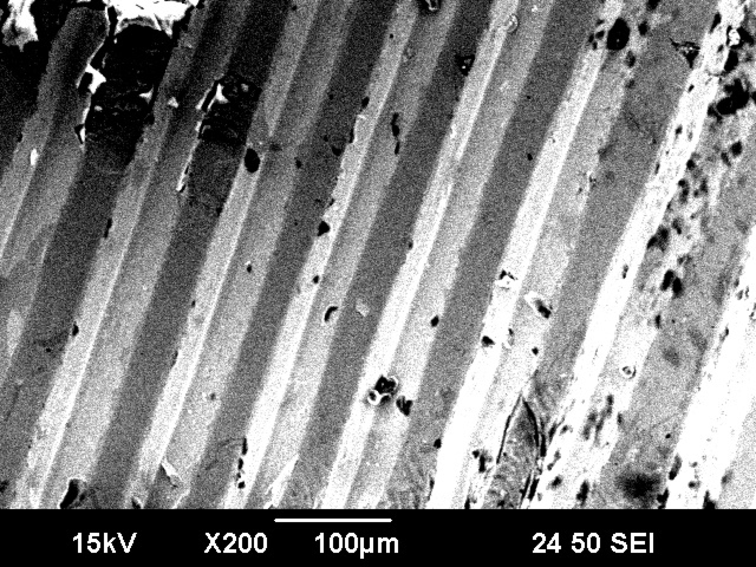
\includegraphics[width=0.85\textwidth]{figs/0523/record/200_15kV.pdf}
    \end{center}
    \caption{200倍 15kV}
  \end{minipage}
\end{figure}

\begin{figure}[H]
  \begin{minipage}{0.5\hsize}
    \begin{center}
      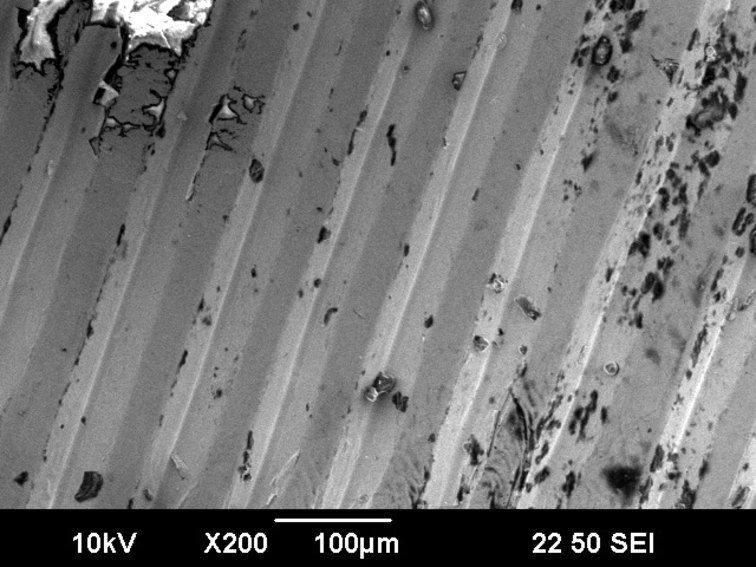
\includegraphics[width=0.85\textwidth]{figs/0523/record/200_10kV.pdf}
    \end{center}
    \caption{200倍 10kV}
  \end{minipage}
  \begin{minipage}{0.5\hsize}
    \begin{center}
      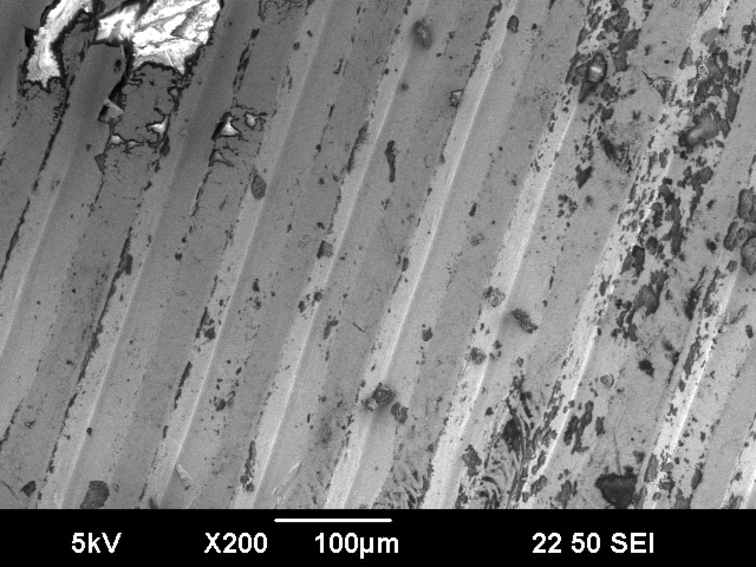
\includegraphics[width=0.85\textwidth]{figs/0523/record/200_5kV.pdf}
    \end{center}
    \caption{200倍 5kV}
  \end{minipage}
\end{figure}

% \subsection{走査型電子顕微鏡による薄膜試料の形態観察}
% 薄膜試料は、基盤の上に数十$\sim$百nmの厚さで形成された薄膜である。その上に、半径の異なる円状の電極が数百nmの大きさで形成されている。\\
% \begin{figure}[H]
%   \begin{minipage}{0.5\hsize}
%     \begin{center}
%       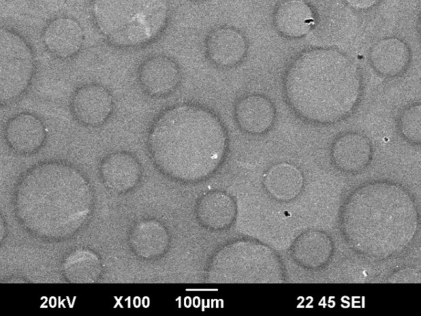
\includegraphics[width=0.85\textwidth]{images/0530pm/0530pm/100_20kV.pdf}
%     \end{center}
%     \caption{薄膜 100倍 20kV}
%   \end{minipage}
%   \begin{minipage}{0.5\hsize}
%     \begin{center}
%       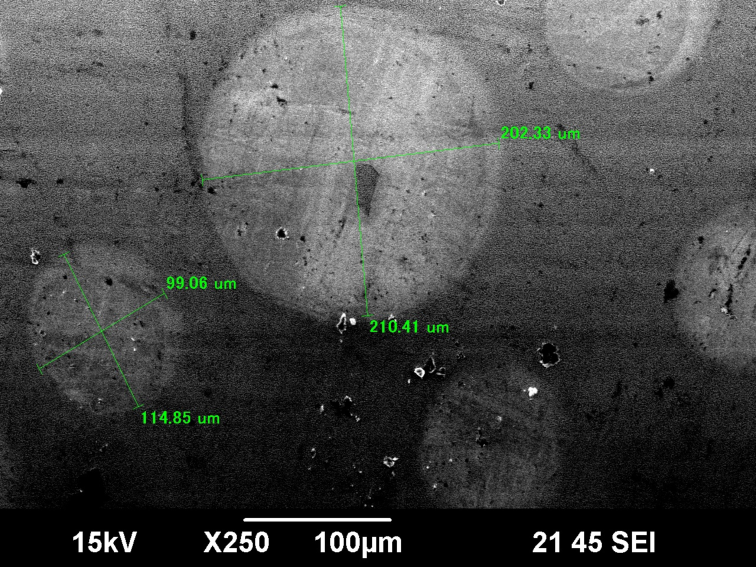
\includegraphics[width=0.85\textwidth]{images/0530pm/0530pm/250_15kv.pdf}
%     \end{center}
%     \caption{薄膜 250倍 20kV}
%   \end{minipage}
% \end{figure}

% \begin{figure}[H]
%   \centering
%   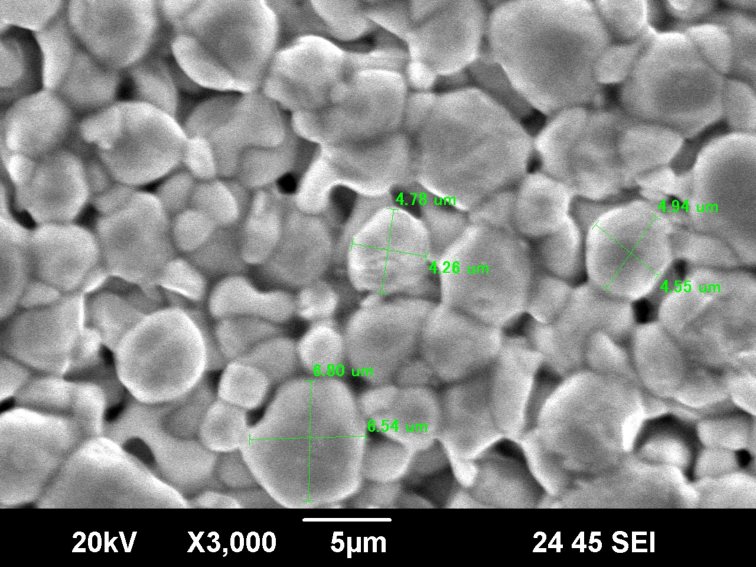
\includegraphics[width=0.425\textwidth]{images/0530pm/bcm3000.pdf}
%   \caption{酸化膜BaCe0.8Y0.2O3-d (BCY) 3000倍 20kV}
% \end{figure}

\section{Discussion}
\subsection{電子顕微鏡の鏡筒内部を真空にする理由}
電子銃から放出した電子が空気分子と衝突せずに試料に到達するためには、電子顕微鏡の鏡筒内部を$10^{-3}\sim 10^{-4}$Paの真空にする必要がある。
空気分子の8割は窒素なので簡略化のため窒素分子で考えることにする。

窒素分子の速度がMaxwell分布に従うと仮定される場合、平均自由行程は
\begin{equation}
  l = \frac{1}{\sqrt{2}n\sigma}
\end{equation}
で表される。
$n$乱源の粒子数密度[\si{m^{-3}}]、$\sigma$は散乱時の有効断面積[\si{m^2}]である。有効断面積とは、粒子が衝突する限界の断面積である。

気体の状態方程式として、気体分子数密度$n$[\si{m^{-3}}]を用いた次式が成り立つ。
\begin{equation}
  p = nk_BT
\end{equation}
$n$について解くと
\begin{equation}
  n = \frac{p}{k_BT}
\end{equation}
となるので、(1)式から
\begin{equation}
  \frac{p}{k_B T} = \frac{1}{\sqrt{2} l\sigma}
\end{equation}
が導かれる。
従って圧力$p$は
\begin{equation}
  p = \frac{k_B T}{\sqrt{2} l\sigma}
\end{equation}
で表される。
窒素分子の直径は$372\times 10^{-12}$ \si{m}であるので、有効断面積は、$\sigma = 4.35\times 10^{-19}$ \si{m^2}となる。
$k_b = 1.38\times 10^{-23} \si{J/K}$、$T$ = 300 \si{K}、平均自由行程は鏡筒の長さ$l = 1$ \si{m}とする。
このとき、圧力$p$は
\begin{equation}
  p = \frac{1.38\times 10^{-23} \times 300}{\sqrt{2} \times 1 \times 4.35\times 10^{-19}} = 6.73\times 10^{-3} \si{Pa}
\end{equation}
となる。
したがって、顕微鏡の観察に必要な真空度は$10^{-2}\sim 10^{-3}$ オーダーであることがわかる。
\subsection{光学顕微鏡と走査型顕微鏡の違い}
光学顕微鏡は可視光領域の電磁波を利用する為、観察対象の色情報を捉えることができる。一方、走査型電子顕微鏡は二次電子の検出量に応じて表面凹凸を白黒の濃淡で再現するため、色情報は含まない。
走査型電子顕微鏡は光学顕微鏡に比べて高い解像度を有するが、観察対象に真空環境が必要であり、制約が存在する。また、光学顕微鏡では焦点深度が限られるが、走査型電子顕微鏡では電子線の波長が短く絞りが小さいため、焦点深度が大きくなることが観察された。
\subsection{走査型電子顕微鏡の傾斜の有無による観察結果の違い}
実験3.1.1の結果の通り、試料を傾けると画像が鮮明になることがわかった。
試料を傾けた場合、一次電子の深度は浅くなる。これは試料が水平の場合と比較して、より表面付近で発生した二次電子の情報を多く反映できることになる為、画像が鮮明になると考えられる。
\subsection{絶縁体試料と伝導性試料における加速電圧の影響}
実験3.2.1の結果の通り、伝導体試料では加速電圧を高くすると解像度が向上することが分かった。
それに対して、実験3.2.2では、絶縁体試料では加速電圧を高くすると解像度が低下することが分かった。
これは、レコード盤は絶縁性試料であり、照射された電子が試料表面に過剰にたまってしまうことが原因であり、
逆に回折格子は伝導性試料であり、電子が試料表面だけでなく試料内部に入っていき、多くの情報をもたらすためであると考えられる。

\section{Conclusion}
実験1では、伝導性試料である回析格子を走査型電子顕微鏡を用いて撮影した。
  実験2では、絶縁性試料であるレコード盤を光学顕微鏡と走査型電子顕微鏡を用いて撮影した。走査型電子顕微鏡では、加速電圧を変化させて撮影した。その結果以下の二つが得られた。一つ目は、導電性試料では、加速電圧を高くすると解像度が向上するが、絶縁性試料では加速電圧を高くすると解像度が低下する。一般に、入射電子のエネルギーを上昇させると二次電子のエネルギーも上昇する為、表面凹凸に応じた二次電子の放出量の差が大きくなる。その結果、濃淡がはっきりと映し出される。しかし、絶縁性試料の場合は、照射された電子が試料表面に過剰にたまってしまう為、加速電圧を高くするほど鮮明さが欠けてしまうと考えられる。\\
  二つ目として、光学顕微鏡では焦点深度が限られるが、走査型電子顕微鏡では電子線の波長が短く絞りが小さいため、焦点深度が大きくなることが観察された。
  
\begin{thebibliography}{文献数}
  \bibitem{ID} 高分子学会, 走査型電子顕微鏡法

\end{thebibliography}

\end{document}